\documentclass[10pt,a4j,twocolumn]{jarticle}
%
\usepackage[dvipdfmx]{graphicx,color,hyperref}
\usepackage{amsmath,amssymb,mathrsfs,amsthm}
\usepackage{ascmac}

\usepackage{centernot}
\usepackage{fancybox}
\usepackage{verbatim}
\usepackage{jtygm}
\usepackage{here,txfonts}
\usepackage{url}
\usepackage{bussproofs}
\usepackage{latexsym}
\usepackage{bm}

\usepackage{proof}

\newcommand\fun[2]{\lambda{#1}.{#2}}

\newcommand\Resetz{\textbf{reset0}}
\newcommand\Shiftz{\textbf{shift0}}
\newcommand\Throw{\textbf{throw}}
\newcommand\resetz[1]{\Resetz~{#1}}
\newcommand\shiftz[2]{\Shiftz~{#1}.{#2}}
\newcommand\throw[2]{\Throw~{#1}~{#2}}

\newcommand\cfun[2]{\underline{\lambda}{#1}.{#2}}

\newcommand\cResetz{\underline{\textbf{reset0}}}
\newcommand\cShiftz{\underline{\textbf{shift0}}}
\newcommand\cThrow{\underline{\textbf{throw}}}
\newcommand\cresetz[1]{\cResetz~{#1}}
\newcommand\cshiftz[2]{\cShiftz~{#1}\to{#2}}
\newcommand\cthrow[2]{\cThrow~{#1}~{#2}}

\newcommand\cPlus{\underline{\textbf{+}}}

\newcommand\cLet{\underline{\textbf{clet}}}
\newcommand\cIn{\underline{\textbf{in}}}
\newcommand\clet[3]{\cLet~{#1}={#2}~\cIn~{#3}}
\newcommand\csp[1]{\texttt{\%}{#1}}
\newcommand\code[1]{\texttt{<}{#1}\texttt{>}}

\newcommand\codeT[2]{\langle{#1}\rangle^{#2}}
\newcommand\contT[2]{({#1} \Rightarrow {#2})}

\newcommand\ord{\ge}

\newcommand\too{\leadsto^*}
\newcommand\pink[1]{\textcolor{pink}{#1}}
\newcommand\red[1]{\textcolor{red}{#1}}
\newcommand\green[1]{\textcolor{green}{#1}}
\newcommand\magenta[1]{\textcolor{magenta}{#1}}
\newcommand\blue[1]{\textcolor{blue}{#1}}

\newcommand\forin[2]{\textbf{for}~{#1}~\textbf{to}~{#2}~\textbf{in}}
\newcommand\cforin[2]{\underline{\textbf{cfor}}~{#1}~\underline{\textbf{to}}~{#2}~\underline{\textbf{in}}}
\newcommand\Let{\textbf{let}}
\newcommand\In{\textbf{in}}
\newcommand\cArray[1]{\underline{[{#1}]}}
\newcommand\cArrays[2]{\underline{[{#1}][{#2}]}}

\usepackage[margin=2.00cm]{geometry}

\usepackage{setspace}
% \setstretch{1.08} % ページ全体の行間を設定
% \setlength{\textheight}{38\baselineskip}
\setlength{\columnsep}{10mm}

\theoremstyle{definition}
\newtheorem{theo}{定理}[section]
\newtheorem{defi}{定義}[subsection]
\newtheorem{lemm}{補題}[section]
\renewcommand\proofname{\bf 証明}

\newcommand{\cn}{\centernot}
\newcommand{\la}{\lambda}
\newcommand{\ri}{\longrightarrow}
\newcommand{\map}{\mapsto}
\newcommand{\id}{\text{id }}

\usepackage{listings,jlisting}
% \usepackage[scale=0.9]{DejaVuSansMono}

\definecolor{DarkGreen}{rgb}{0,0.5,0}
\definecolor{Magenta}{rgb}{1.0, 0.0, 1.0}

\lstset{
  language={[Objective]Caml},% プログラミング言語
  basicstyle={\ttfamily\small},% ソースコードのテキストのスタイル
  keywordstyle={\bfseries},% 予約語等のキーワードのスタイル
  commentstyle={},% コメントのスタイル
  stringstyle={},% 文字列のスタイル
  frame=none,% ソースコードの枠線の設定 trlb (none だと非表示)
  numbers=none,% 行番号の表示 (left だと左に表示)
  numberstyle={},% 行番号のスタイル
  xleftmargin=5pt,% 左余白
  xrightmargin=5pt,% 右余白
  keepspaces=true,% 空白を表示する
  mathescape,% $ で囲った部分を数式として表示する ($ がソースコード中で使えなくなるので注意)
  % 手動強調表示の設定
  moredelim=[is][\itshape]{@/}{/@},
  moredelim=[is][\color{red}]{@r\{}{\}@},
  moredelim=[is][\color{blue}]{@b\{}{\}@},
  moredelim=[is][\color{DarkGreen}]{@g\{}{\}@},
  moredelim=[is][\color{Magenta}]{@m\{}{\}@}
}

\title {\vspace{-2.0cm}多段階 let 挿入を行うコード生成言語の設計}
\date{2016年7月12日}
\author{システム情報工学研究科 コンピュータサイエンス専攻 \\
  博士課程前期2年 201520621 大石純平 \\
  指導教員 亀山幸義
}


% \pagestyle{empty}

\begin{document}

\maketitle
% \thispagestyle{empty}
\section{はじめに}
コード生成法は,プログラムの生産性・保守性と実行性能の高さを両立させられるプログラミング手法として有力なものである.
本研究室では,コード生成法をサポートするプログラム言語の信頼性・安全性を高める研究を行ってきている.
本研究は,コード生成法で必要とされる「多段階let挿入」等を簡潔に表現できるコントロールオペレータである shift0/reset0を持つコード生成言語とその型システムを構築し,生成されたコードの型安全性を保証する.

% すなわち,プログラム生成を行うことによって生成されるプログラムが安全に
% 実行されることを,プログラムの生成段階より早い段階,
% すなわちプログラム生成を行うプログラムのコンパイル段階で検査することの
% できる言語体系およびシステムを構築することを目標としている.

多段階let挿入は,入れ子になったforループを飛び越えたコード移動を許す仕組みであり,ループ不変式の移動などのために必要である.

ここでいう安全性は,構文的に正しいプログラムであること,
文字列同士の加算や乗算を決して行わない等の通常の型安全性を満たすことのほか,
自由変数やプログラム特化後において利用できない変数に依存したプログラム
を生成しないという,変数や変数スコープに関する性質を含む概念である.

この研究での大きな課題は,従来のコード生成のためのプログラミング言語の多くが,純粋なラムダ計算に基づく関数型プログラミング言語を基礎としており,効率の良いコードを生成する多くの技法をカバーしていないことである.これを克服する体系,すなわち,効率良いプログラムを記述するための表現力を高めつつ,安全性が保証された体系が求められている.

本研究の目的は,安全性が厳密に保証される計算体系の理論を構築し,さらにそれを実現する処理系を実装することを目的とする.このため,比較的最近になって理論的性質が解明されつつあるshift0/reset0 というコントロールオペレータに着目し,これをコード生成の体系に追加して得られた体系を構築して,上記の課題を解決することを狙いとする.

コード生成言語の型安全性に関して,破壊的代入を持つ体系に対する須藤らの研究\cite{Sudo2014}等があるが,本研究は,彼らの環境識別子に対する小さな拡張により,shift0/reset0 に対する型システムが構築できることを示す.

\section{準備}
\subsection{マルチステージプログラミング}
マルチステージプログラミングとはプログラムを生成する段階や,生成したプログラムを実行する段階など,複数のステージを持つプログラミングの手法である.
プログラムを計算対象のデータとして扱うことで,プログラムの効率や,保守性,再利用性の両立が期待できる.
例えば生成元のプログラムから,何らかの目的に特化したプログラムを生成を行い,保守や改変をしたい時は,生成元のプログラムに対して行えばよいので,生成後のコードについては手を加える必要が無い.そのような,マルチステージプログラミングを効果的に行うためには,言語レベルで,プログラムを生成,実行などが行える機構を備えることが望ましい.
そのような言語のことをコード生成言語と呼ぶ.
% そのような言語として,本研究では,MetaOCamlというマルチステージプログラミングに対応したOCamlの拡張言語を用いる.

\subsection{shift0/reset0}
継続を扱う命令としてコントロールオペレータというものがある.継続とは,計算のある時点における残りの計算のことである.本研究では,shift0/reset0というコントロールオペレータを用いる.
reset0は継続の範囲を限定する命令であり,shift0はその継続を捕獲するための命令である.

shift/reset\cite{Danvy1990}では,複数の計算エフェクトを含んだプログラムは書くことができない.しかし,階層化shift/resetやshift0/reset0はこの欠点を克服している.
階層化shift/reset\cite{Danvy1990}は,最大レベルの階層を固定する必要があるが,shift0/reset0では,shift0,reset0 というオペレータだけで,階層を表現する事ができるという利点がある.
また,shift0/reset0は shift/reset よりも単純なCPS変換で意味が与えられていて,純粋なラムダ式で表せるために形式的に扱いやすいという利点がある.
我々の言語体系において,コードを扱うreset0は $\cResetz ~M$というように表し,これは,継続の範囲を$M$に限定するという意味である.
コードを扱うshift0は $\cShiftz ~k ~\to ~M$というように表し,これは,直近のreset0によって限定された継続を $k$ に束縛し,$M$ を実行するという意味である.
つまり,shift0 と reset0 は対応関係にあり,reset0で切り取った継続を,shift0によって,$k$ へと束縛し,その継続を使うことができるようになる.

shift/reset\cite{Danvy1990} は,直近のreset による限定継続のスコープからひとつ上のスコープまでしか,継続を捕獲することができないが,shift0/reset0においては,直近の reset0内のスコープだけでなく,遠くの,reset0 で限定された継続を捕獲することができる.そのことによって,本研究の肝である多段階let挿入が可能となる.

以下で,我々の言語体系におけるshift0/reset0 による多段階let挿入の例を掲載する.

\begin{align*}
    e &= \red{\cResetz} ~~\cLet~x_1=\csp{3}~\cIn \\
      &\phantom{=}~~ \blue{\cResetz} ~~\cLet~x_2=\csp{5}~\cIn \\
      &\phantom{=}~~ \blue{\cShiftz}~\blue{k_2}~\to~ \red{\cShiftz}~\red{k_1}~\to~ \magenta{\cLet~y=t~\cIn} \\
      &\phantom{=}~~ \cThrow~\red{k_1}~(\cThrow~\blue{k_2}~(x_1~\cPlus~x_2~\cPlus~y))
\end{align*}

まず,
$\blue{\cResetz}$によって,切り取られた継続 $\cLet~x_2=\csp{5}~\cIn$ が,
$\blue{\cShiftz}$ によって,$\blue{k_2}$へと捕獲され,
次に,
$\red{\cResetz}$によって,切り取られた継続 $\cLet~x_2=\csp{3}~\cIn$ が,
$\red{\cShiftz}$ によって,$\red{k_1}$へと捕獲される.

わかりやすいところまで計算を進めると以下のようになり,
\begin{align*}
  e & \too \magenta{\cLet~y=t~\cIn} \\
    & \phantom{\too}~~ \cThrow~\red{k_1}~(\cThrow~\blue{k_2}~(x_1~\cPlus~x_2~\cPlus~y))
\end{align*}

$\magenta{\cLet~y=t~\cIn}$ がトップに挿入されたことが分かる.
$\cThrow$ は,切り取られた継続を引数に適用するための演算子である.
つまり,
\begin{align*}
  e & \too \magenta{\cLet~y=t~\cIn} \\
    & \cLet~x_1=\csp{3}~\cIn \\
    & \cLet~x_2=\csp{5}~\cIn \\
    & (x_1~\cPlus~x_2~\cPlus~y)
\end{align*}

となり,$\magenta{\cLet~y=t~\cIn}$ が 二重の $\cLet$を飛び越えて,挿入された事が分かる.
このような操作は,shift/reset では不可能であり,階層的な shift0/reset0 であるからできることである.

\section{目的}
プログラムによるプログラムの動的な生成を行い,保守性と性能の両立をはかりたい.
また,生成するプログラムだけでなく,生成されたプログラムも型の整合性が静的に(生成前に)保証するようにしたい.

コード生成のアプローチとしては,
コード生成のプログラムは,高レベルの記述つまり,高階関数,代数的データ型などを利用し,抽象的なアルゴリズムの記述を行う.
それによって生成されたコードは低レベルの記述がなされており高性能な実行が可能となる.また,特定のハードウェアや特定のパラメータを仮定したコードなので,様々な環境に対して対応できる.

つまり,生成元のプログラムは抽象度を上げた記述をすることで,色々な状況(特定のハードウェア,特定のパラメータ)に応じたプログラムを生成することを目指す.
そのようにすることで,生成後のコードには手を加えることなく,生成前のプログラムに対してのみ保守や改変をすれば良い.
また,プログラム生成前に型検査に通っていれば,生成後のコードに型エラーは絶対に起こらないことが,型システムにより,保証される.

しかし,コード生成において以下の様な信頼性への大きな不安がある.

\begin{itemize}
\item 構文的,意味的に正しくないプログラムを生成しやすい
\item デバッグが容易ではない
\item 効率のよいコード生成に必要な計算エフェクト(今回の場合だと限定継続のひとつであるshift0/reset0)を導入すると,従来理論ではコード生成プログラムの安全性は保証されない
\end{itemize}

効率のよいコードの生成を行うためには例えば,ネストしたループの順序の入れ替えやループ不変項,共通項のくくりだしなどを行う必要がある.
それらを実現するためには,コード生成言語に副作用が必要である.

\section{研究項目}
表現力と安全性を兼ね備えたコード生成の体系としては,
2009年の亀山らの研究\cite{Kameyama2009}が最初である.
彼らは,MetaOCamlにおいてshift/resetとよばれるコントロールオペレータを
使うスタイルでのプログラミングを提案するとともに,
コントロールオペレータの影響が変数スコープを越えることを制限する型シス
テムを構築し,安全性を厳密に保証した.
% Westbrookら\cite{Westbrook}は同様の研究を Java のサブセットを対象におこなった.
須藤ら\cite{Sudo2014}は,書換え可能変数を持つコード生成体系に対して,
部分型付けを導入した型システムを提案して,安全性を保証した.
これらの体系は,安全性の保証を最優先した結果,表現力の上での制限が強く
なっている.特に,let挿入とよばれるコード生成技法をシミュレートするた
めには,shift/reset が必要であるが,複数の場所へのlet挿入を許すために
は,複数の種類のshift/resetを組み合わせる必要がある.
この目的のため,階層的shift/resetやマルチプロンプト
shift/resetといった,shift/reset を複雑にしたコントロールオペレータを
考えることができるが,その場合の型システムは非常に複雑になることが予想
され,安全性を保証するための条件も容易には記述できない,等の問題点がある.

本研究では,このような問題点を克服するため,shift/reset の意味論をわず
かに変更した shift0/reset0 というコントロールオペレータに着目する.
このコントロールオペレータは,長い間,研究対象となってこなかったが
2011年以降,Materzok らは,部分型付けに基づく型システムや,
関数的なCPS変換を与えるなど,簡潔で拡張が容易な理論的基盤をもつことを
解明した\cite{Materzok2011,materzok2012}.
特に,shift0/reset0 は shift/reset と同様のコントロールオペレータであ
りながら,階層的shift/reset を表現することができる,という点で,
表現力が高い.本研究では,これらの事実に基づき,これまでのshift/reset
を用いたコード生成体系の知見を,shift0/reset0 を用いたコード生成体系の
構築に活用するものである.

\section{本研究の手法}
shift0/reset0 を持つコード生成言語の型システムの設計を須藤らの研究\cite{Sudo2014}を元に行い,深く入れ子になった内側からの,let挿入,assertion挿入の関数プログラミング的実現を目指すのだが,shift0/reset0 は shift/resetより強力であるため,型システムが非常に複雑である.
また,コード生成言語の型システムも一定の複雑さを持っている.
そのためにそれらを単純に融合させることは困難である.

そこで,本研究では,コード生成の言語に shift0/reset0を組み合わせた言語を設計し,その言語によって書かれたプログラムの安全性は,型システムで安全なコードには型がつくように,安全でないコードには型がつかないように,型システムを構築する.
須藤らの\cite{Sudo2014}の環境識別子 Environment Classifier による型による変数のスコープのアイデアを拡張することによって,shift0/reset0の型安全性を保証する.
% 型システムの安全性の保証に関しては,Kameyama+ 2009\cite{Kameyama2009} と Sudo+ 2014\cite{Sudo2014} の手法を利用する.

\section{本研究の型システム}

\subsection{型付け例}
\begin{align*}
  e & = \cResetz ~~\cLet~x_1=\csp{3}~\cIn \\
    & \phantom{=}~~ \cResetz ~~\cLet~x_2=\csp{5}~\cIn \\
    & \phantom{=}~~ \cShiftz~k_2~\to~ \cShiftz~k_1~\to~ \red{\cLet~y=t~\cIn} \\
    & \phantom{=}~~ \cThrow~k_1~(\cThrow~k_2~(x_1~\cPlus~x_2~\cPlus~y))
\end{align*}

$e$の計算を進めると以下のようになる.

\begin{align*}
  e & \too \red{\cLet~y=t~\cIn} \\
    & \phantom{\too}~~ \cResetz ~~\cLet~x_1=\csp{3}~\cIn \\
    & \phantom{\too}~~ \cResetz ~~\cLet~x_2=\csp{5}~\cIn \\
    & \phantom{\too}~~ (x_1~\cPlus~x_2~\cPlus~y)
\end{align*}

$t=\csp{7}$ のとき $e_2$ は型が付く

$t=x_2$ か $t=x_1$ のとき $e_2$ は型が付かない

$t$によって,安全なコードか安全でないコードかが変わるので,それを型で判断したい.
このような型システムを構築することを考える.

\subsection{環境識別子 EC によるスコープ表現\cite{Sudo2014}}
コードレベルの変数スコープと,型によるスコープの表現を表したのが下の図である.

\begin{center}
  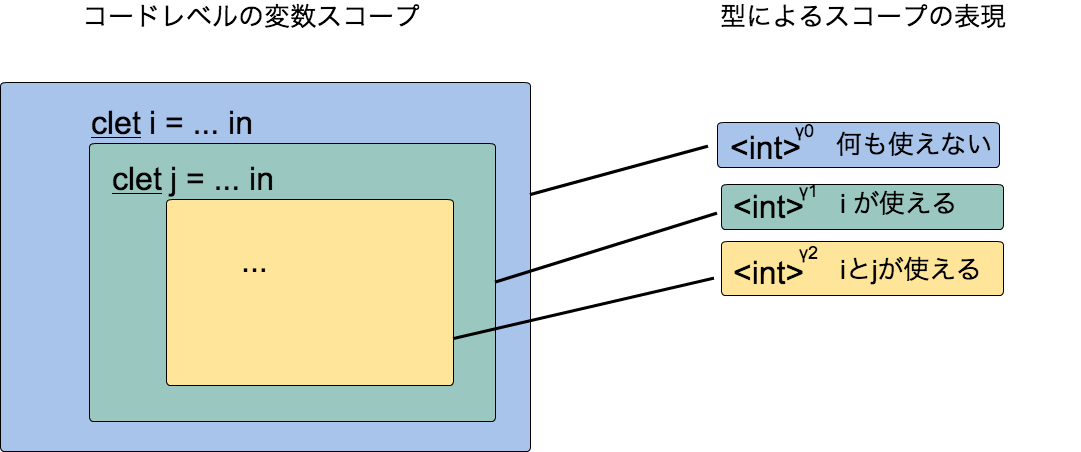
\includegraphics[clip,height=3.5cm]{./img/eccletin.png}
\end{center}

$\gamma$は変数のスコープを表し,そのスコープ内で使える自由変数の集合と思ってもらえば良い.
$\gamma$には,包含関係があり,それを $\gamma_1 \ord \gamma_0$ というような順序で表す.
直感的には$\gamma_0$より$\gamma_1$のほうが使える自由変数が多いという意味である.

このように EC を型に付加することで,その型がどのスコープに存在するかどうかが分かる.

\subsection{EC の洗練化}
今までは,プログラムがネストしていけば,その分だけ,使える自由変数が増えていたのだが,shift0/reset0が導入されたことにより,計算の順序が変わることがあり,単純にネストした分だけ使える自由変数が増えていくという訳にはいかない.

下の図は,
\begin{align*}
  & \cLet~ i = ...~\cIn \\
  & \cResetz ~~\cLet~ j = ...~\cIn \\
  & \Shiftz~ k~ \to~ \cLet~y=t~\cIn \\
  & \Throw~ k ...
\end{align*}
のスコープに色を付け,計算結果とともに載せた図である.
また,下のグラフは ECの順序を視覚的に表している図である.

\begin{center}
  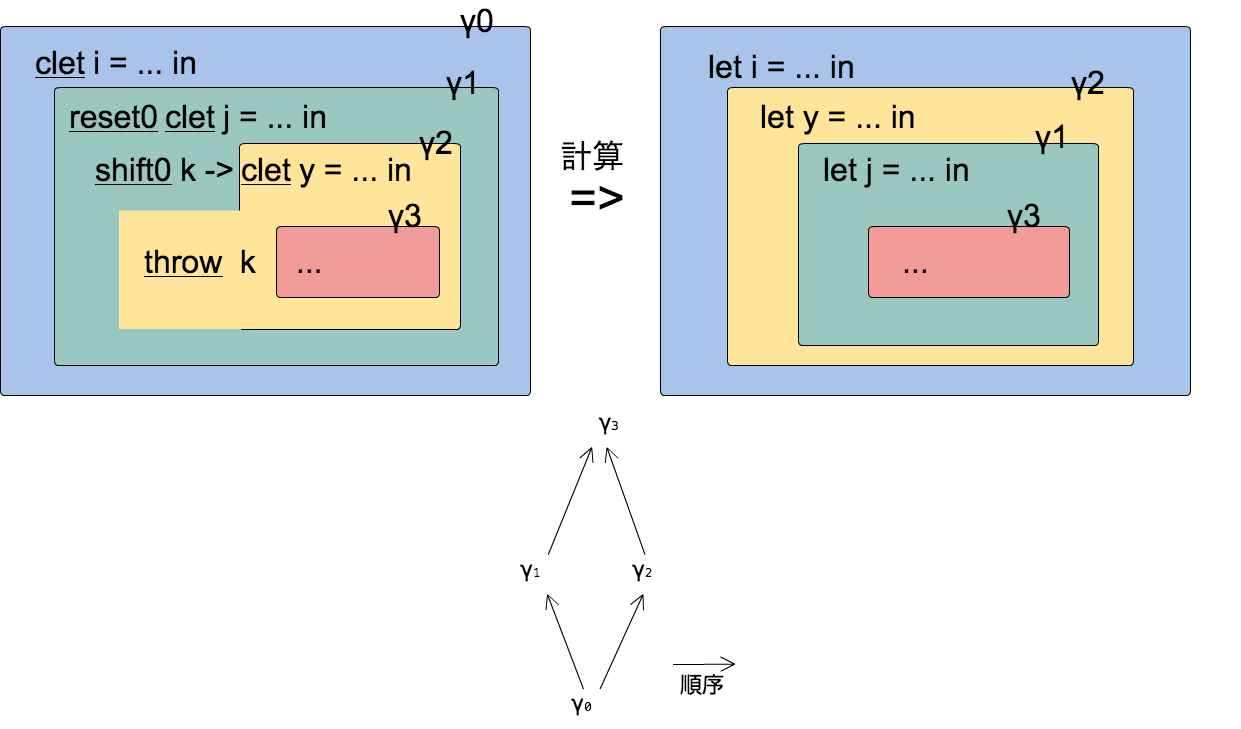
\includegraphics[clip,height=4.5cm]{./img/resume_ecex.png}
\end{center}
計算を進めると,reset0 によって,切り取られた継続がshift0によって $k$へ捕獲され, throw によって,使用されることにより,計算の順序が変わり,計算後では$\gamma_1$ と $\gamma_2$ のスコープの包含関係が入れ替わっている事がわかる.

\subsection{EC のジョイン}
今までの,ECでは,計算の順序が変わることが無かったので,継続を任意の場所に貼り付けることを安全に行うことができなかった.しかし,ECのジョインというものを考えることで,shift0/reset0を用いたlet挿入のコード生成の型安全性の保証を行うことができる.

\begin{center}
  
\includegraphics[clip,height=4cm]{./img/ecgraph.png}
\end{center}

上図は下のことを視覚的に表したグラフである.
\begin{itemize}
\item $\gamma_1$ のコードレベル変数は $\gamma_2$ では使えない
\item $\gamma_2$ のコードレベル変数は $\gamma_1$ では使えない
\item $\gamma_1, \gamma_2$ のコードレベル変数は $\gamma_3$ で使える
\end{itemize}

$\cup$という概念を追加することで,shift0/reset0を用いたlet挿入のコード生成の型安全性の保証を行うことができる.

\section{まとめと今後}
多段階let挿入がshit0/reset0で記述可能なことを実例によって提示した.また,shift0/reset0を導入した言語を考えると従来より,簡潔で,検証しやすい体系ができるというアイデアに基づいて,コード生成言語の型システムを構築することを提案した.
コード生成言語の型システム\cite{Sudo2014}に shift0 reset0 を組み込んだ 型システムの設計を行い,その型システムによって型が付く場合と付かない場合の例をみた.

今後,設計した型システムの健全性の証明 (subject reduction 等)を行い,および型検査器等の実装を行う.

%% 参考文献
\addcontentsline{toc}{section}{参考文献}
\bibliography{../bib/bibfile}
\bibliographystyle{junsrt}

\end{document}

%%% Local Variables:
%%% mode: japanese-latex
%%% TeX-master: t
%%% End:
